\section{Differential Equations}
\subsection{Poisson's equation}

This it the introduction ~\cite{Example}.

A first demonstration is solving the Poisson equation, which is elliptic. For a domain
$ \Omega \subset \mathbb{R}^n $ with boundary $\partial \Omega = \Gamma_{D} \cup \Gamma_{N}$ the equation reads:

\begin{align}
  -\nabla^2 u   &= f  && \text{in $\Omega$,} \\
      u   &= 0  && \text{on $\Gamma_D$,} \\
  \nabla u \cdot n &= g  && \text{on $\Gamma_N$.}
\end{align}

\subsection{hp-FEM}
An extension of finite elements are the hp-finite-elements, which use quadratic elements, of width $h$, and a sum of consecutive polynomial functions of degree $p$, used as the test function.


\section{Neural Networks}
Neural nets have had many successes with many computational problems in the last few years, thanks to their ability to very quickly and in a parallel way to optimize certain problems. ~\cite{Example}

\begin{figure}[!ht]
  \centering
  \tikzset{%
  every neuron/.style={
    circle,
    draw,
    minimum size=0.65cm
  },
  neuron missing/.style={
    draw=none,
    scale=3,
    text height=0.222cm,
    execute at begin node=\color{black}$\vdots$
  },
}

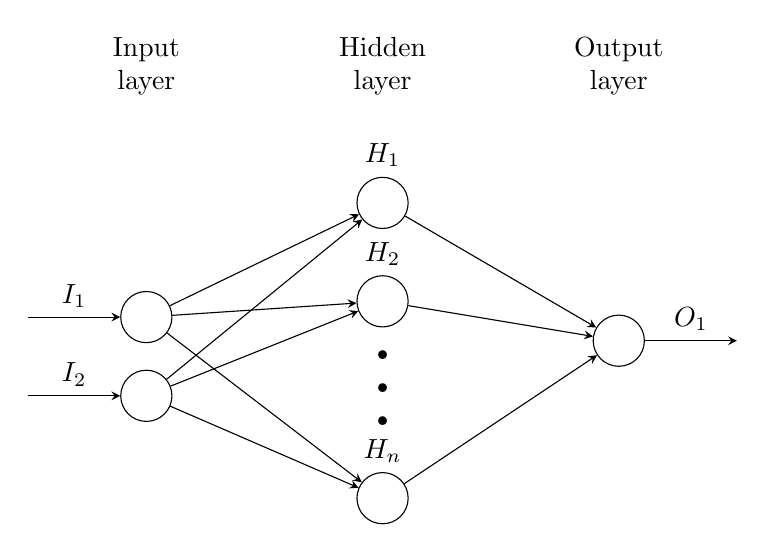
\begin{tikzpicture}[x=1.5cm, y=1.0cm, >=stealth]

\foreach \m/\l [count=\y] in {1,2}
  \node [every neuron/.try, neuron \m/.try] (input-\m) at (0,0.3-\y) {};

\foreach \m [count=\y] in {1,2,missing,3}
  \node [every neuron/.try, neuron \m/.try ] (hidden-\m) at (2,2-\y*1.25) {};

\foreach \m [count=\y] in {1}
  \node [every neuron/.try, neuron \m/.try ] (output-\m) at (4,0.0-\y) {};

\foreach \l [count=\i] in {1,2}
  \draw [<-] (input-\i) -- ++(-1,0)
    node [above, midway] {$I_\l$};

\foreach \l [count=\i] in {1,2,n}
  \node [above] at (hidden-\i.north) {$H_\l$};

\foreach \l [count=\i] in {1}
  \draw [->] (output-\i) -- ++(1,0)
    node [above, midway] {$O_\l$};

\foreach \i in {1,2}
  \foreach \j in {1,2,...,3}
    \draw [->] (input-\i) -- (hidden-\j);

\foreach \i in {1,2,...,3}
  \foreach \j in {1}
    \draw [->] (hidden-\i) -- (output-\j);

\foreach \l [count=\x from 0] in {Input, Hidden, Output}
  \node [align=center, above] at (\x*2,2) {\l \\ layer};

\end{tikzpicture}

\end{figure}

\subsection{Automatic Differentiation}

\subsection{Physics Informed Neural Networks}

Due to the overlap of the notation of "test" within Finite Element Analysis and Machine Learning,
to avoid any confusion in this work we will use the former unless explicitly told so.
